Ci-dessous, un graphe qui montre la différence entre le coût obtenu, pour un certain epsilon et pour une certaine légère modification de la demande, via la procédure présentée à la question 4 et le coût obtenu en résolvant complètement le problème avec les données initiales modifiées. Sur le graphe la différence est normalisée en pourcentage par rapport au résultat obtenu via la seconde méthode. Chaque point vaut:
\begin{equation*}
difference = \frac{resultat_{dual} - resultat_{reecriture}}{résultat_{reecriture}} * 100 
\end{equation*}
 
\begin{figure}[h]
    \centering
    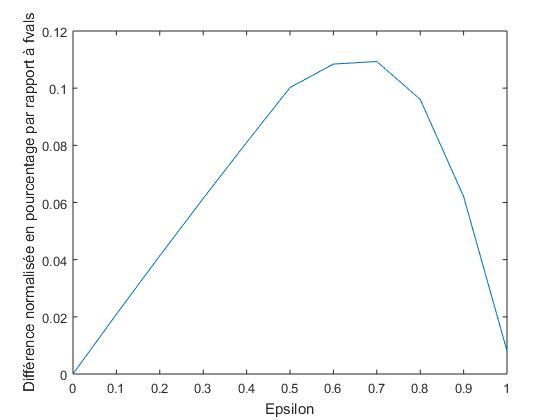
\includegraphics[width=0.8\textwidth]{graphes/graphq5.jpg}
    \caption{Graphe de la production à personnel constant}
    \label{fig:q5}
\end{figure}

La différence entre les deux méthodes dépasse à peine les 0,1\%. C'est négligeable à l'échelle utilisée ici. La procédure présentée à la question 4 est donc suffisante.